% https://sagroups.ieee.org/1916-1/pve-sdn/ieee-pve-sdn-2022/cfp2022/
\documentclass[conference]{IEEEtran}
\IEEEoverridecommandlockouts
% The preceding line is only needed to identify funding in the first footnote. If that is unneeded, please comment it out.
\renewcommand*\ttdefault{txtt}
\usepackage[inline]{enumitem}
\usepackage{cite}
\usepackage{amsmath,amssymb,amsfonts}
\usepackage{algorithmic}
\usepackage{graphicx}
\usepackage{textcomp}
\usepackage[dvipsnames,table]{xcolor}
\usepackage{booktabs}
\usepackage[utf8]{inputenc}
\usepackage[english]{babel}
\usepackage{todonotes}
\usepackage{multirow}
\usepackage{amssymb} % For the checkmark
\usepackage{amssymb} % For the checkmark
\usepackage{graphicx} % For the rotation
\usepackage{array} % To enlarge the vertical space of the table's contents
\usepackage{amssymb}% http://ctan.org/pkg/amssymb
\usepackage{pifont}% http://ctan.org/pkg/pifont
\usepackage{longtable}
\newcommand{\cmark}{\ding{51}}%
\newcommand{\xmark}{\color{red!75}\ding{55}}%
\usepackage{amsmath}
\usepackage{cleveref} %package for section and subsection
\crefformat{section}{\S#2#1#3} % see manual of cleveref, section 8.2.1
\crefformat{subsection}{\S#2#1#3}
\crefformat{subsubsection}{\S#2#1#3}


\def\BibTeX{{\rm B\kern-.05em{\sc i\kern-.025em b}\kern-.08em
    T\kern-.1667em\lower.7ex\hbox{E}\kern-.125emX}}


%%% comments -begin
\usepackage{amsfonts,amsmath,amssymb,amstext,latexsym}
\usepackage{ifthen}
\newboolean{showcomments}
\setboolean{showcomments}{true} %false true
\ifthenelse{\boolean{showcomments}}
{ \newcommand{\mynote}[3]{
    \fbox{\bfseries\sffamily\scriptsize#1}
    {\small$\blacktriangleright$\textsf{\emph{\color{#3}{#2}}}$\blacktriangleleft$}}}
{ \newcommand{\mynote}[3]{}}
\newcommand{\shrink}[1]{}
\newcommand{\h}[1]{\mynote{Haruna}{#1}{Purple}}
\newcommand{\dimitrios}[1]{\mynote{Dimitrios}{#1}{RoyalBlue}}
\newcommand{\y}[1]{\mynote{Yehia}{#1}{blue}}
%%% comments - end

%%% table stuff
\newcommand{\midsepremove}{\aboverulesep=0mm \belowrulesep=0mm}
\midsepremove
\newcommand{\midsepdefault}{\aboverulesep=0.02mm \belowrulesep=0.15mm}
\midsepdefault
\definecolor{rowcolor}{RGB}{204,221,245}
\newcommand{\rc}{\rowcolor{rowcolor}}

\usepackage{balance}

\usepackage{thmtools}
\declaretheorem[
    name=Takeaway,
    shaded={bgcolor=Peach!20,padding=2pt,rulecolor=Maroon,rulewidth=0.5pt},
]{summary}

\begin{document}

\title{On the Performance Benefits of Heterogeneous Virtual Network Function Execution Frameworks}

\author{\IEEEauthorblockN{Haruna Umar Adoga}
\IEEEauthorblockA{\textit{School of Computing Science}\\
\textit{University of Glasgow}\\
Glasgow, UK\\
h.adoga.1@research.gla.ac.uk}
\and
\IEEEauthorblockN{Yehia Elkhatib}
\IEEEauthorblockA{\textit{School of Computing Science}\\
\textit{University of Glasgow}\\
Glasgow, UK\\
yehia.elkhatib@glasgow.ac.uk}\\
\and
\IEEEauthorblockN{Dimitrios P. Pezaros}
\IEEEauthorblockA{\textit{School of Computing Science}\\
\textit{University of Glasgow}\\
Glasgow, UK\\
dimitrios.pezaros@glasgow.ac.uk}

}
\maketitle

\begin{abstract}
As the adoption of softwarized network functions (NFs) 
keeps growing, we evaluate the performance benefits of SDN-aware data-plane implementations when compared to diverse acceleration and process-based NFV frameworks. Typical network functions have been implemented using four alternative frameworks scenarios, an SDN-aware software switch (data-plane), a virtual machine (VM), a Data-Plane Development Kit (DPDK) NF, and a containerized NF. Results from our experiments show that the data-plane NF implementation yields much higher bandwidth and packets per second (pps) rates. The bandwidth obtained is 14\% more than the user-space scenario while retaining CPU utilization. The DPDK NFs in our evaluation can process packets at a much higher rate for 64B packets, on a single CPU core, which is 7 times higher than the containerized NF implementations, also tied to a single core. Our results also show the performance gains from deploying virtual network functions on heterogeneous frameworks.
\end{abstract}


\begin{IEEEkeywords}
SDN, Data-plane, Network Function Virtualization, Network Softwarization, Containerized Network Functions, DPDK, Virtual Network Functions, Virtual Machines, Performance Comparison, NFV frameworks.
\end{IEEEkeywords}

%%%%%%%%%%%%%%%%%%%%%%%%%%%%%%%%%%%%%%%%%%%%%%%%%%%%%%%%%%%%%%%%%%%%%%%%%%%%%
%%%%%%%%%%%%%%%%%%%%%%%%%%%%%%%%%%%%%%%%%%%%%%%%%%%%%%%%%%%%%%%%%%%%%%%%%%%%%
\section{Introduction}
\label{Introduction}
The flexibility offered by network function virtualization (NFV) and software-defined networking SDN allows service providers to deploy Virtual Network Functions (VNFs) in a flexible and scalable manner, with the simple goal of meeting the packet processing requirements of applications. The important components that must be present for NFV to be implemented are: 
\begin{enumerate*}[label=(\roman*)]
    \item the NFV Infrastructure (NFVI), which consists of a virtualization layer for hosting VNFs;
    \item the abstracted network function, which runs on the NFVI; 
    \item the NFV Management and Orchestration framework (NFV-MANO) for the management and orchestration of virtualized resources and the VNF lifecycle \cite{asquini2021etsi}.
\end{enumerate*}

The data-plane of the network serves as a suitable alternative for implementing VNFs. Hence network operators can leverage the data-plane as well as process-based NFV frameworks for deploying softwarized network functions.
Doing so comes with the benefit of cost reduction on procuring high-end servers for NFV deployment, and reduction also on the overheads for compute-bound network functions (Table \ref{VNF-Table}). 
Typically, VNF deployment is carried out using 
VMs~\cite{qureshi2022network}, 
containers~\cite{huang2021novel}, 
Unikernels~\cite{wang2022performance}, 
Click-based processing elements, 
and Data-Plane Development Kit (DPDK) which uses zero-copy and kernel bypass to speed up packet processing \cite{zhang2016opennetvm}. 

At the same time, service providers need to understand how to leverage the network data-plane for the deployment of network functions. In this paper, we carry out a practical performance evaluation on a real testbed to compare the implementation of representative network functions as part of an SDN-aware data-plane against having such functionality abstracted and implemented as a VNF running on a commodity server -- using heterogeneous VNF execution frameworks. One of the problems is to find out where to best implement these functions, which should allow for faster service deployments and for specific applications to be deployed using the suitable processing pipeline in the network.

We make the following contributions:
\begin{itemize}
    \item We present a classification of virtual network functions (Table \ref{VNF-Table}) based on the type of operations they perform on packets. After motivating the need for data-plane NF deployments, we designed a testbed that is suitable for getting comparative results (for both scenarios, i.e., software switch and separate virtualized functions on commodity servers).
    
    \item A significant difference in the performance of heterogeneous virtualized packet processing frameworks was identified. We achieved this by carefully evaluating packets of various sizes at the data-plane, compared to having equivalent network functions on commodity servers. 
    
    \item Our discussion in \cref{NFclassification} and \cref{Discussion} sheds light on what network functions are suitable for both scenarios, based on our evaluation. We analyzed and presented our findings, with packet processing acceleration frameworks, using Intel DPDK and lightweight containers, which shows a significant improvement in the performance of the network functions evaluated.
\end{itemize}

Next, we present the design of the testbed used for the first performance evaluation, which also contains a classification of network functions and their complexity. The evaluation of both scenarios is presented in Section~\ref{evaluations}. A high-performance setup and the results obtained using this approach are presented in Section~\ref{dpdk}, with DPDK and Docker containers. In Section~\ref{Discussion}, we shed some light on what network functions are ideal for deployment using the environments considered, including some design implications. We present related work in Section~\ref{Related Work}, and conclude the work in Section~\ref{conclusion}. 



%%%%%%%%%%%%%%%%%%%%%%%%%%%%%%%%%%%%%%%%%%%%%%%%%%%%%%%%%%%%%%%%%%%%%%%
\begin{table*}[ht]
\caption{Virtual Network Functions Operations and Classification}
\begin{center}
\begin{tabular}{cccc}
\toprule
\textbf{VNF} & \textbf{Description} & \textbf{Compute-bound} & \textbf{I/O-bound}\\
\midrule
DPI -- IDS/IDP & Traffic logging and inspection, stateful/stateless security &\cmark &\xmark\\
%\midrule
\rc Virtual Private Network & User traffic encryption and security &  \cmark & \xmark\\
%\midrule
 Network Address Translation (NAT) & Private to public IP translation and vice versa &\cmark & \xmark\\
%\midrule
\rc WAN Optimizer & ISP traffic optimization for QoS & \cmark & \xmark \\
%\midrule
Router & Packet routing based on L3 details &  \cmark &\xmark\\
%\midrule
\rc L2 Switch & Packet switching based on MAC addresses  &  \cmark &\xmark\\
%\midrule
Load Balancer & Traffic load balancing, based on application level policies & \xmark & \cmark\\
%\midrule
\rc ACL/Firewall & Device or application level access control &\xmark & \cmark\\
Caching & Performance improvements for better QoS/QoE &  \xmark& \cmark \\
%S\midrule
\rc IPv4/IPv6 proxy & IPv4 to IPv6 connections proxy &\xmark & \cmark\\
%S\midrule
Header Classifier & Classification, based on IP header fields & \xmark& \cmark\\
%\midrule
\bottomrule
\end{tabular}
\label{dataset}
\label{VNF-Table}
\end{center}
\end{table*}
%%%%%%%%%%%%%%%%%%%%%%%%%%%%%%%%%%%%%%%%%%%%%%%


%%%%%%%%%%%%%%%%%%%%%%%%%%%%%%%%%%%%%%%%%%%%%%%%%%%%%%%%%%%%%%%%%%%%%%%
\section{Design - VNF Classification and Complexity}
\label{NFclassification}
In Table \ref{VNF-Table}, we capture some of the most popular NFs that can be abstracted and implemented in software, and their classification as discussed below.
We classify NFs based on how they process packets and the typical operations they carry out along the processing pipeline. We use Figure \ref{FirewallNF} to illustrate how packets traverse representative NFs that perform similar operations on received packets, such as an ACL/ Firewall. These NFs perform IP header lookups to read fields such as source and destination addresses and port numbers, and the protocol in use. In the case of an ACL/Firewall, packets are checked against predefined match-action rules to either discard or forward them. 

Figure \ref{DPI} illustrates the typical mode of operation of the second group of representative NFs (Table \ref{VNF-Table}), i.e., NFs that perform operations beyond basic packet header lookup against predefined match-action rules. Packets traversing these NFs go through more fine-grained inspection of payload data, depending on the type of NF. A typical operation might involve performing regex matches, compression parameters for Quality of Service optimizations or encryption parameters.

We arrived at the conclusion of Table \ref{VNF-Table} after carefully considering the behavior of virtual network functions and frameworks that were implemented in notable works such as \cite{kulkarni2018reinforce, perino2014caesar, adoga2022network, chen2022automatic}, where representative virtual network functions such as IDS/DPIs and L3 routers exhibit compute-bound characteristics, while others such as ACL/firewalls are I/O-bound due to the nature of operations they carry out on packets traversing them \cite{katsikas2018metron, bremler2016openbox}.

\begin{figure}[tb]
\centering
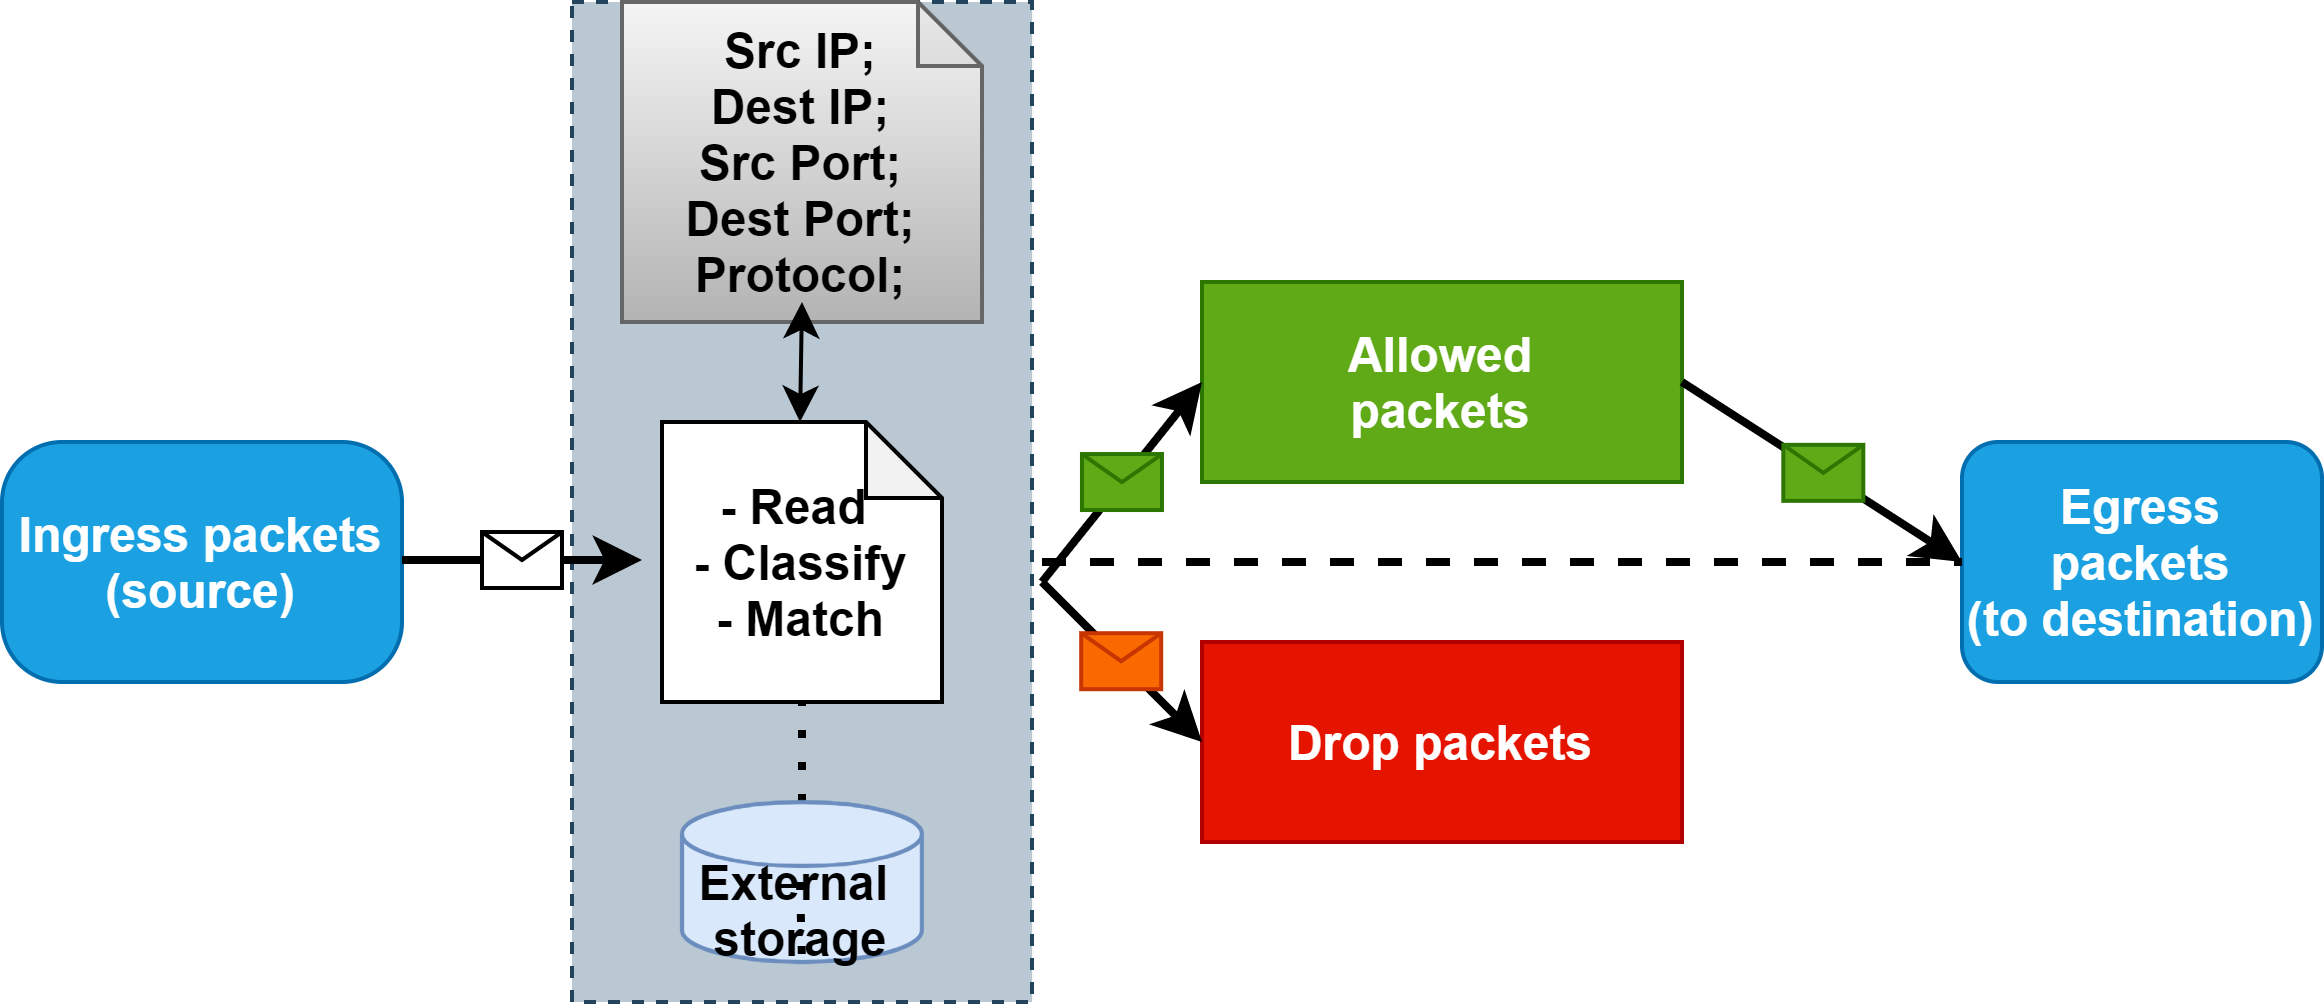
\includegraphics[width=\columnwidth]{FirewallNF.png}
% 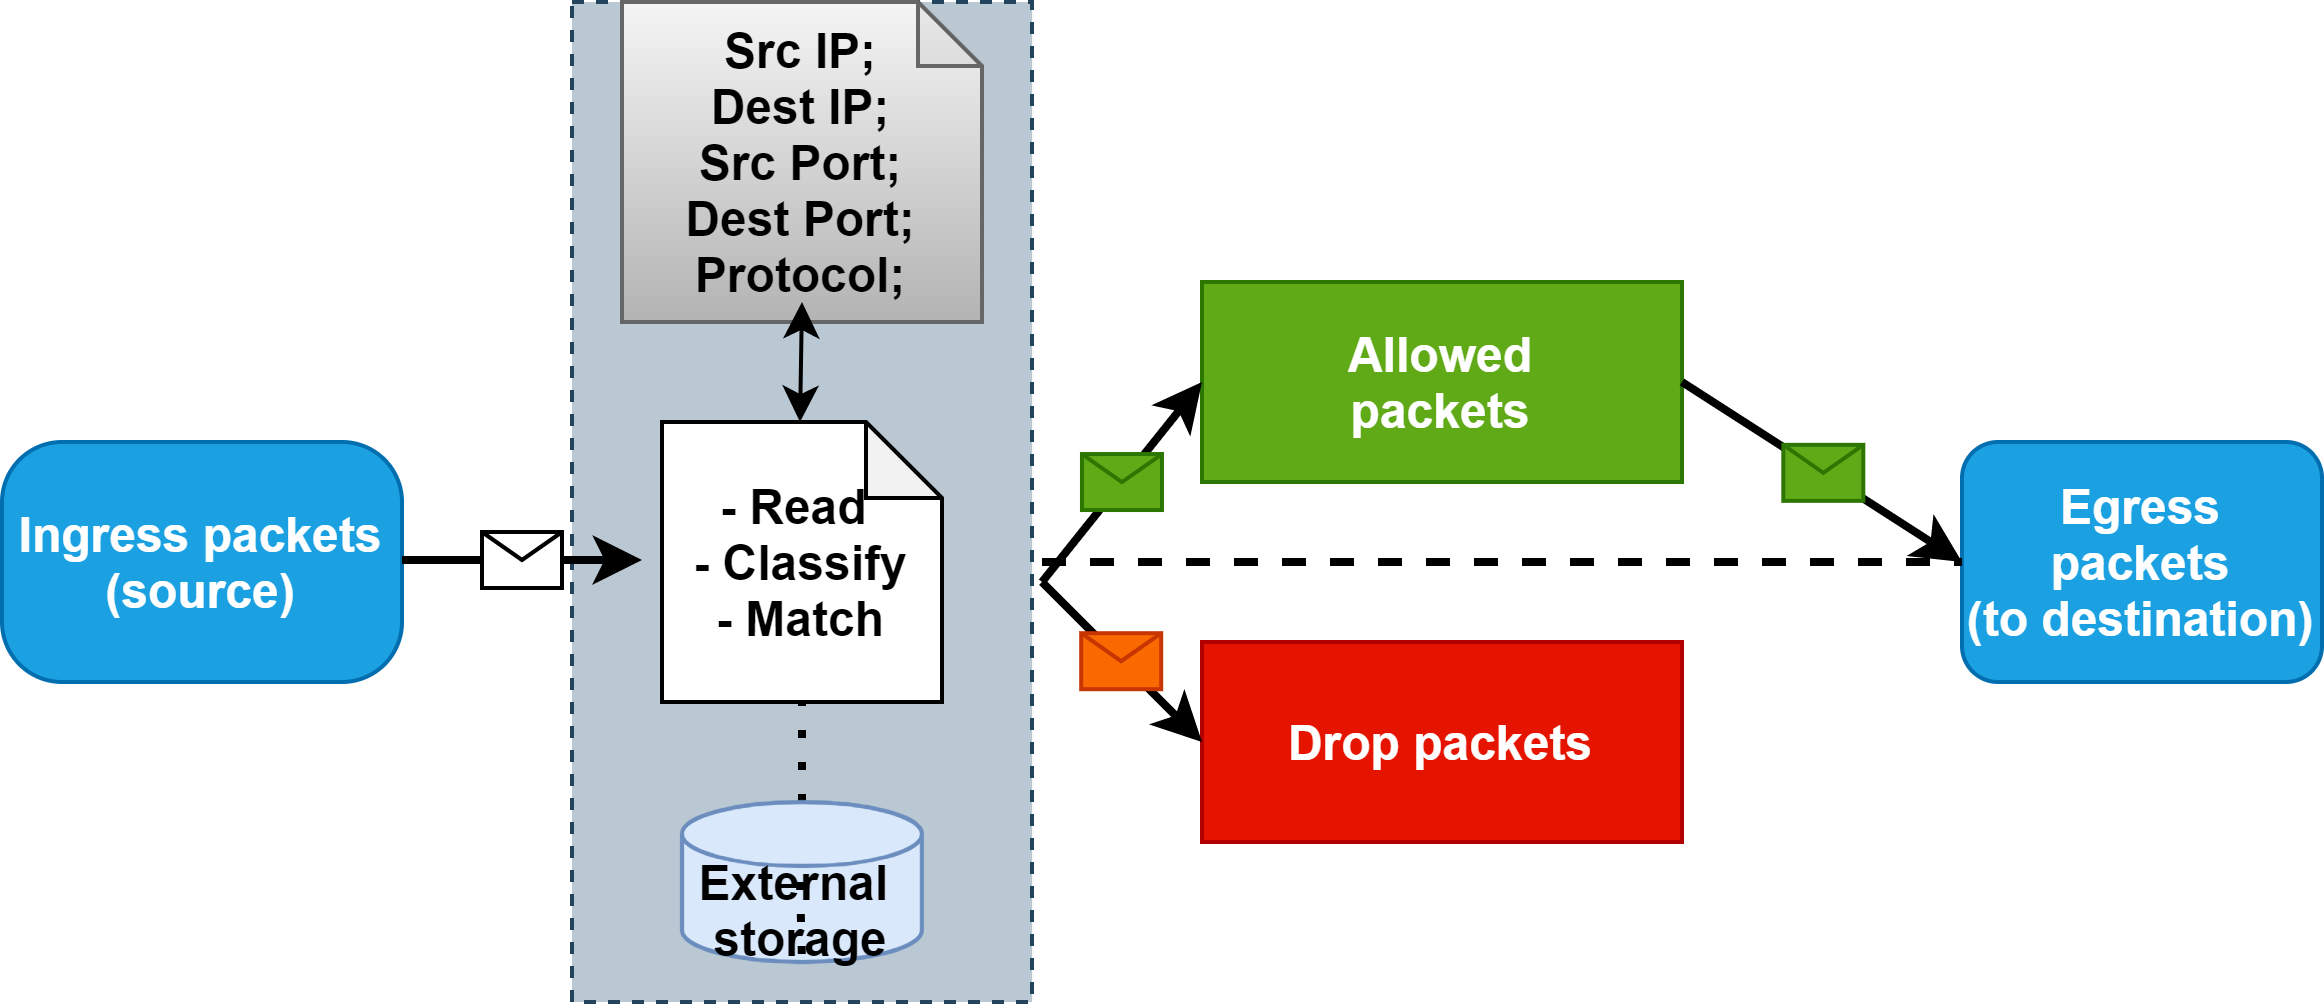
\includegraphics[width=80mm,scale=2.0]{FirewallNF.png}
\caption{An overview of the operation of I/O-bound NFs, e.g., ACL/Firewall, Header Classifier, and caching. Their tasks involve IP header lookup and data store access.}
\label{FirewallNF}
\end{figure}

\begin{figure}[tb]
\centering
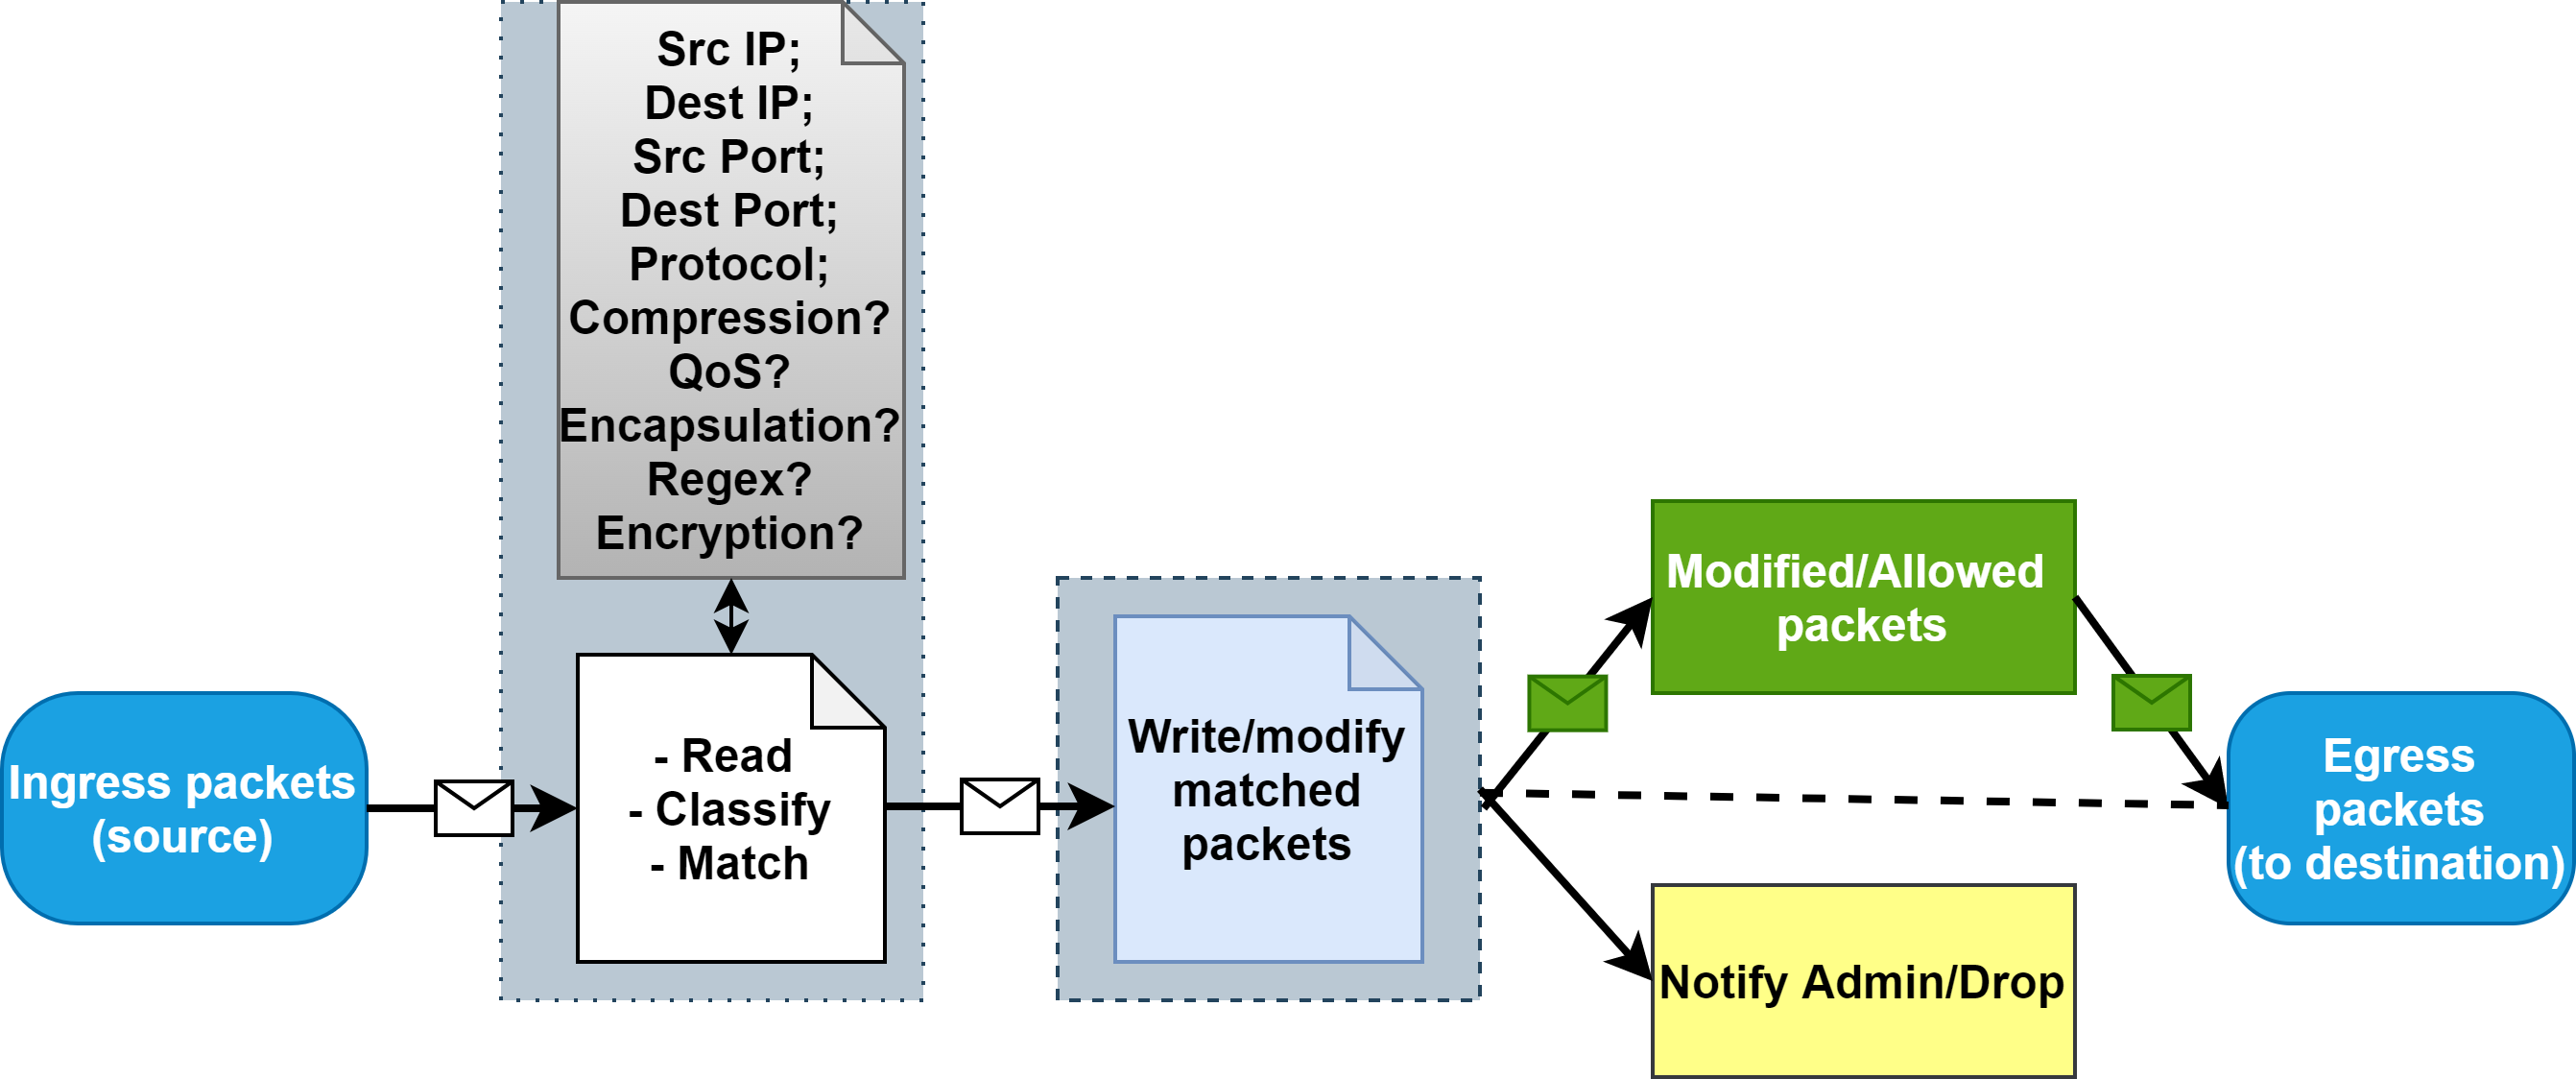
\includegraphics[width=\columnwidth]{DPI.png}
% 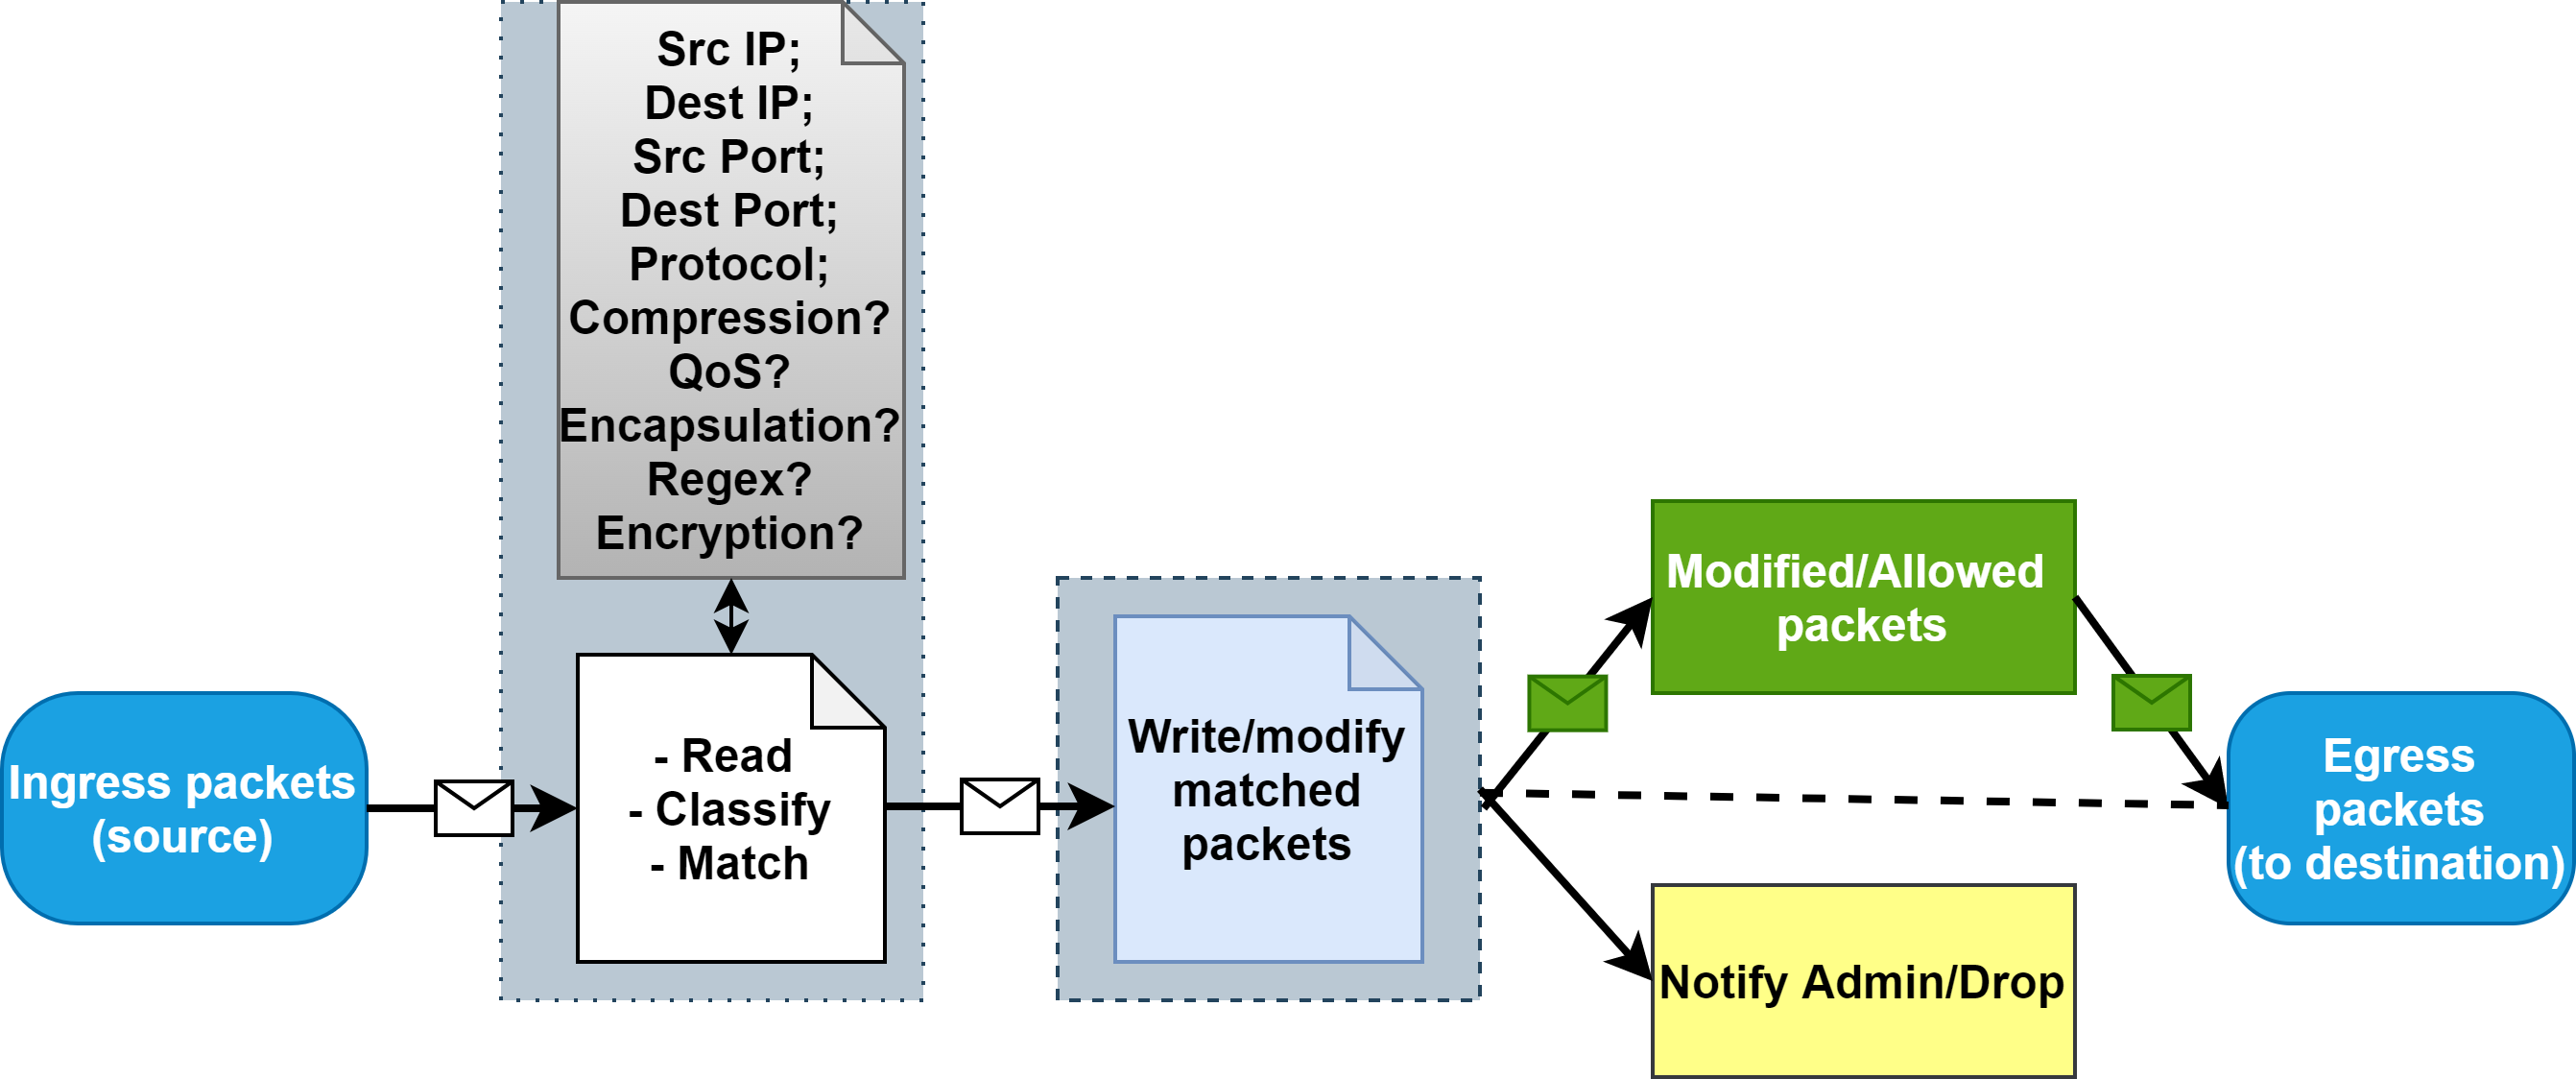
\includegraphics[width=80mm,scale=2.0]{DPI.png}
\caption{An overview of the operation of compute-bound NFs, e.g., NAT, IDS and QoS optimization. Their tasks involve more complex types of processing performed on packets.}
\label{DPI}
\end{figure}
%%%%%%%%%%%%%%%%%%%%%%%%%%%%%%%%%%%%%%%%%%%%%%%%%%%%%%%%%%%%%%%%%%%%%%

 Answering the question about what network functions are suitable for data-plane deployments is important, because the SDN-aware data-plane has some limitations alongside benefits in terms of its capabilities which we explore in the remainder of the paper.
%%%%%%%%%%%%%%%%%%%%%%%%%%%%%%%%%%%%%%%%%%%%%%%%%%%%%%%%%%%%%%%%%%%%%%%%%%%%%%%%%%%%%%%%%
%%%%%%%%%%%%%%%%%%%%%%%%%%%%%%%%%%%%%%%%%%%%%%%%%%%%%%%%%%%%
\subsection{Testbed design}
\label{design}

We describe the testbed we designed to evaluate the performance of heterogeneous VNF execution frameworks.
We started our design first by identifying the NFs that can be equally deployed at the data-plane level of an SDN-aware software switch and as a separate user-space VNF entity in the network. Looking at Table~\ref{VNF-Table}, with their typical mode of operation and complexity in mind, NFs that are I/O-bound can be deployed using both approaches for a fair evaluation. Also, for any significant performance degradation/improvement to be observed, at least two different VNF implementations can produce comparable results. %, i.e., we should be able to deduce, using some NFs from Table~\ref{VNF-Table}. 

Two typical scenarios are a Longest Prefix Match (LPM) router and a stateless firewall that, on the one hand, are configured using predefined match-action rules on a virtual switch, and on the other hand having the same functionalities running as separate entities (i.e. VNFs) in the network. This aspect of our testbed represents the required abstracted NF component of the ETSI NFV specification \cite{asquini2021etsi}.

%%%%%%%%%%%%%%%%%%%%%%%%%%%%%%%%%%%%%%%%%%%%%%%%%%%%%%%
\subsection{Virtual switches}
SDN-aware virtual switches such as the Open~vSwitch (OvS) have a data-plane component that handles traffic forwarding. In terms of NFV implementations, the network data-plane can be represented using a production-grade virtual switch \cite{tu2021revisiting}. Virtual switches can be configured to emulate typical middlebox functionalities such as firewall/access control, Network Address Translation (NAT), routing, and switching. When functioning as a router, it matches the longest source and destination IP prefix and forwards packets, using specified ports. Firewall functionality matches IP addresses and specific TCP/UDP port numbers, and denies or permits packets (based on match-action flow rules).
%%%%%%%%%%%%%%%%%%%%%%%%%%%%%%%%%%%%%%%%%%%%%%%%%%%%%%%%%%%%
% \subsubsection{Data-plane scenario using a virtual switch}
\subsection{Data-plane scenario design}
\label{Data-plane Setup}
For performance reasons, hosting all VNFs (middleboxes) in a single server can lead to resource contention \cite{saxena2022ofp}. This informed our decision to isolate the NFs from the packet generator (Figure \ref{OvS Testbed}) by making use of multiple (two) physical servers in our first testbed. We investigated both NFs using two servers which are connected back-to-back to also eliminate overheads that are caused by switches. NIC speeds were set to 1000Mbps for consistency throughout our evaluations.
 
The testbed is depicted in Figure \ref{OvS Testbed}. We configured an OvS virtual switch on a physical server running Linux kernel 5.4.0-59-generic, on Ubuntu 20.04 (DUT in Figure \ref{OvS Testbed}). The CPU is an Intel\textregistered{} Core\texttrademark{} i7-8700 @ 3.20GHz, with 6 CPU cores. Virtual interfaces are set to 1GB speeds for the software switch scenario. For the firewall NF configuration, up to 15 different match-action firewall rules were pre-installed on the virtual switch to process HTTP (port 80) traffic that is destined for the web-server or the FTP server (ports 20 and 21) at any given time in our scenario. Paravirtualised (virtio-net) NICs were used on the VMs for better performance. Packets destined for the HTTP and FTP servers were filtered to allow or drop, based on protocol type, data link and transport layer protocols. We reused the same setup for the router NF tests this time by creating match-action rules to route packets coming from the packet generator and destined for the FTP and HTTP service based on layer 3 information using LPM lookup. 

%%%%%%%%%%%%%%%%%%%%%%%%%%%%%%%%%%
\begin{figure}[htbp]
\centering
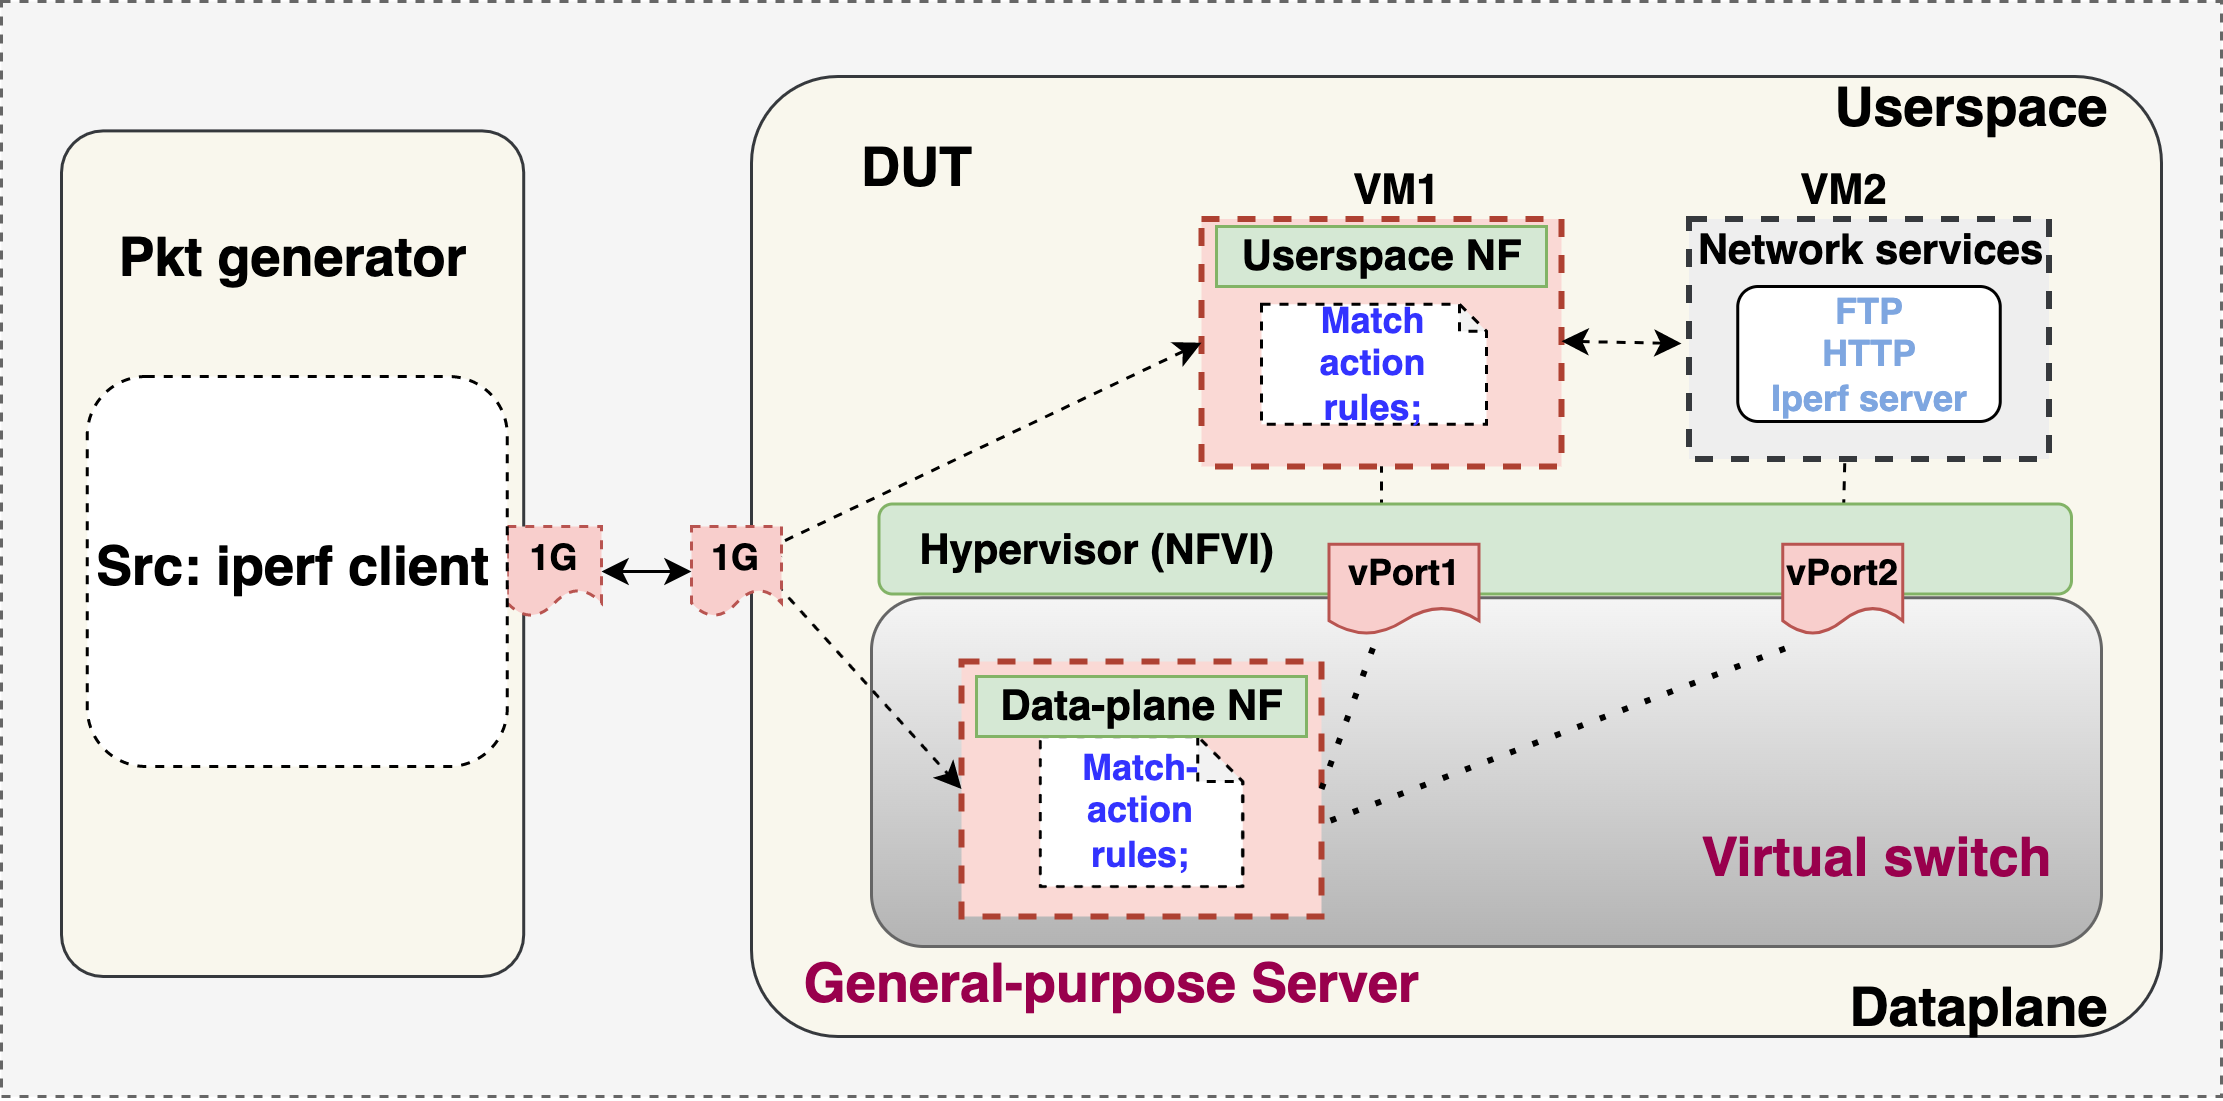
\includegraphics[width=0.92\columnwidth]{OVStestbed.png}
\caption{Ingress packets destined for the FTP and HTTP services on VM2, are made to traverse the data-plane or user-space network function at any given time. User-space function runs on VM1 while data-plane rules are inserted on the virtual switch.}
\label{OvS Testbed}
\end{figure}
%%%%%%%%%%%%%%%%%%%%%%%%%%%%%%%%%
 




\subsection{VNF scenario design}
\label{VNF-setup-section}
 For a comparable scenario to be achieved, the commodity server (DUT) hosting the network functions setup as our NFVI is the same server used for the data-plane scenario (\cref{Data-plane Setup}). VMs running on Kernel-based Virtual Machine (KVM) with minimal versions of the Linux kernel 3.10.0 were used, with virtual network interfaces set to 1GB speeds. We configured a kernel-based firewall function on VM1, an implementation of equivalent functionality to the data-plane firewall rules in terms of the operations carried out on received packets, i.e., matching packets based on source and destination ports or IP addresses. A simple webserver rendering a webpage on port 80 and an FTP server listening on ports 20 and 21 (VM2) is also configured to receive requests. We configured the router NF, a simple Linux kernel-based router to route packets between two separate networks, with the packet generator and DUT server connected back to back (Figure \ref{OvS Testbed}).

%%%%%%%%%%%%%%%%%%%%%%%%%%%%%%%%%%%%%%%%%%%%%%%%%%%%%%%%%%%%%%
%%%%%%%%%%%%%%%%%%%%%%%%%%%%%%%%%%%%%%%%%%%%%%%%%%%%%%%%%%%%%%
\section{Assessing Virtual Network Functions Performance}
\label{evaluations}
We now present the results from the first testbed in our work, described in the previous section.
We measure representative performance parameters such as throughput, packet rate and CPU utilization for each scenario. The presented bandwidth measurements in Figure~\ref{PPSsingle} are averaged over 10 runs each using \texttt{iperf3} (varying the \texttt{len} option to accommodate different packet sizes). 


\subsection{Data-plane performance}
The supported bandwidth achieved on the data-plane firewall scenario was observed to be only 226Mbps for 64B packets. Meanwhile, the largest packets (1500B) were transferred at a bandwidth of 957Mbps, which is about 96\% of the line rate. The data-plane router NF can process 185Mbps at small packet size (64B), and 905Mbps for large ones (1500B). To put the results into perspective, 
Table \ref{bandwidthsummary} and Figure \ref{PPSsingle} summarize the bandwidth for the data-plane and user-space implementations of firewall and router NFs, with various packet sizes. 
The data-plane implementation outperforms the user-space scenario, yielding about 14\% more bandwidth for 1500B packets (Figure \ref{PPSsingle}). 
Both NFs (router and firewall) produced a reasonably high bandwidth when compared with the user-space VNF implementations. 
The drop in performance, which was observed with small packet sizes is due to the increase in packet-per-second processing rate, which is seen as a drawback in most software-based middleboxes.

%%%%%%%%%%%%%%%%%%%%%%%%%%%%%%%%%%
\begin{figure}[htbp]
\centering
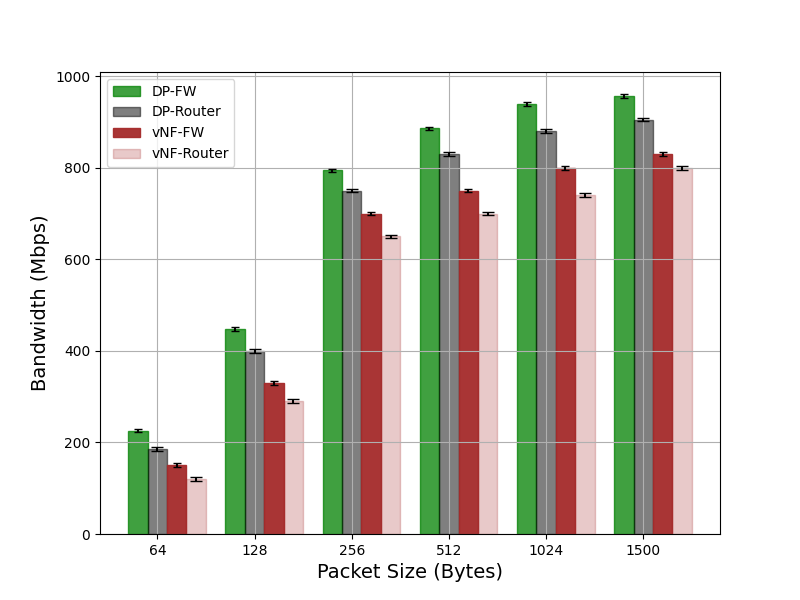
\includegraphics[width=0.9\columnwidth]{PPSdouble1.png}
\caption{Mean bandwidth rates for data-plane and user-space deployments of network functions. The data-plane functions (both firewall and router), consistently outperforms user-space functions in this scenario.}
\label{PPSsingle}
\end{figure}

%%%%%%%%%%%%%%%%%%%%%%%%%%%%%%%%%%%%%%%%%%%%%%%%%%%%%%%%%%%%%%%%%%%%%
\begin{table}[tbp]
\caption{Mean bandwidth rates (in Mbps) for data-plane and VNF deployments.
}
\centering
\begin{tabular}{c|rrrr}
\toprule
\textbf{Packet size (B)} & \textbf{DP-FW} & \textbf{VNF-FW} & \textbf{DP-Router} & \textbf{VNF-Router}\\
\midrule
64 &      226 &  150  & 185 & 120   \\
\rc 128 & 448 & 330   & 400 & 290 \\
256   &   794 & 700   & 750 & 650 \\
\rc 512 & 886 & 750   & 830 & 700 \\
1024    & 939 & 800   & 880 & 740 \\
\rc 1500  & 957 & 830 & 905 & 800 \\
\bottomrule
\end{tabular}%
\label{bandwidthsummary}
\end{table}

 %%%%%%%%%%%%%%%%%%%%%%%%%%%%%%%%%%%%%%%%%%%%%%%%%%%%%%%%%%%%%%%%%%%%%%%%%%%%%%%
\subsection{VNF performance}
\label{vnfperformance}
Like the data-plane scenario, the performance while sending various packet sizes to the HTTP and FTP services with packets traversing the user-space network function %, in the first instance 
was measured and plotted in Figure~\ref{PPSsingle}. 
With the firewall functionality in place and the client machine (packet generator) attempting to gain access to the server hosting the services (VM2), the bandwidth peaked at 150Mbps (for 64B packets), which is a significant decrease from 226Mbps observed in the data-plane scenario. Similar tests were carried out for the router NF, producing a bandwidth of 120Mbps for 64Bytes packets. MTU-sized packets produced 800Mbps, which is about about 11\% below the bandwidth reached in the corresponding data-plane router scenario i.e, 905Mbps. 

For MTU-sized packets, bandwidth of 830Mbps (for the firewall NF scenario) was achieved, which is 13\% less than the data-plane firewall scenario. For this first set of experiments, we observed that the data-plane scenarios outperform our user-space VNF implementations, in terms of maximum bandwidth and CPU utilization, this also holds true for the packets per second rates (Figure \ref{PPSsingle}). 

CPU utilization of the commodity server hosting the testbed is depicted in Figure \ref{PhysicalCPU}, which gives the processing cost of having the NFs deployed in both scenarios. 
By implication, in terms of CPU utilization cost, the data-plane implementation of our firewall requires less resources.

 The CPU utilization for VNF and data-plane scenarios were observed for the router and firewall NFs used in our evaluations. CPU spikes were much higher in the firewall VNF scenario (up to 120\%, which is exactly 10\% of the overall CPU cores on the server. Higher CPU utilization was achieved for smaller packet sizes, which decreases as packet size increases (Figure \ref{PhysicalCPU}).
 
\begin{figure}[htbp]
\centering
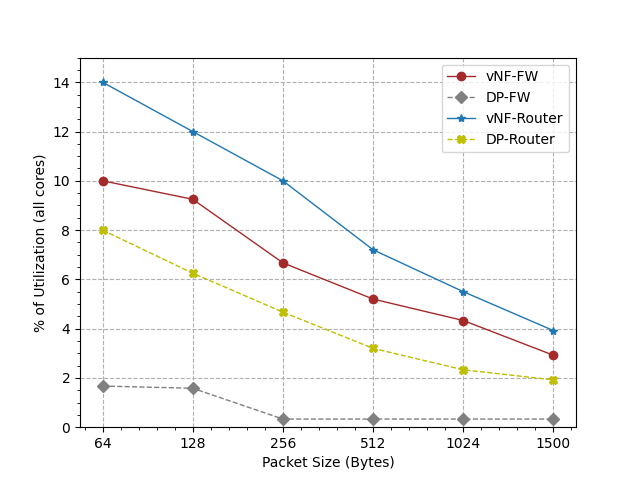
\includegraphics[width=0.8\columnwidth]{PhysicalCPU.png}
\caption{CPU utilization of the DUT -- data-plane firewall and router (grey and yellow lines) maintain much lower CPU utilization, when compared with user-space functions (blue and red lines).}
\label{PhysicalCPU}
\end{figure}



%%%%%%%%%%%%%%%%%%%%%%%%%%%%%%%%%%%%%%%%%%%%%%%%%%%%%%%%%%%
%%%%%%%%%%%%%%%%%%%%%%%%%%%%%%%%%%%%%%%%%%%%%%%%%%%%%%%%%%%%%



%%%%%%%%%%%%%%%%%%%%%%%%%%%%%%%%%%%%%%%%%%%%%%%%%%%%%%%%%%%%%%%%%%
%%%%%%%%%%%%%%%%%%%%%%%%%%%%%%%%%%%%%%%%%%%%%%%%%%%%%%%%%%%%%%%%%%
\subsection{DPDK And Containerised Network Functions}
\label{dpdk}
In this section, we present our findings using an implementation that handles line-rate packet generation and processing. This helps in finding out the behaviour of the same representative network functions on a high performance vNF execution framework and lightweight containers. We carried out this part of the experiment using the Intel Data-Plane Development Kit (DPDK)\footnote[1]{https://www.dpdk.org/} framework and compared the packet processing rates with containerized NFs scenario which involves the deployment of the same network function on Docker containers. 

\begin{figure}[ht]
\centering
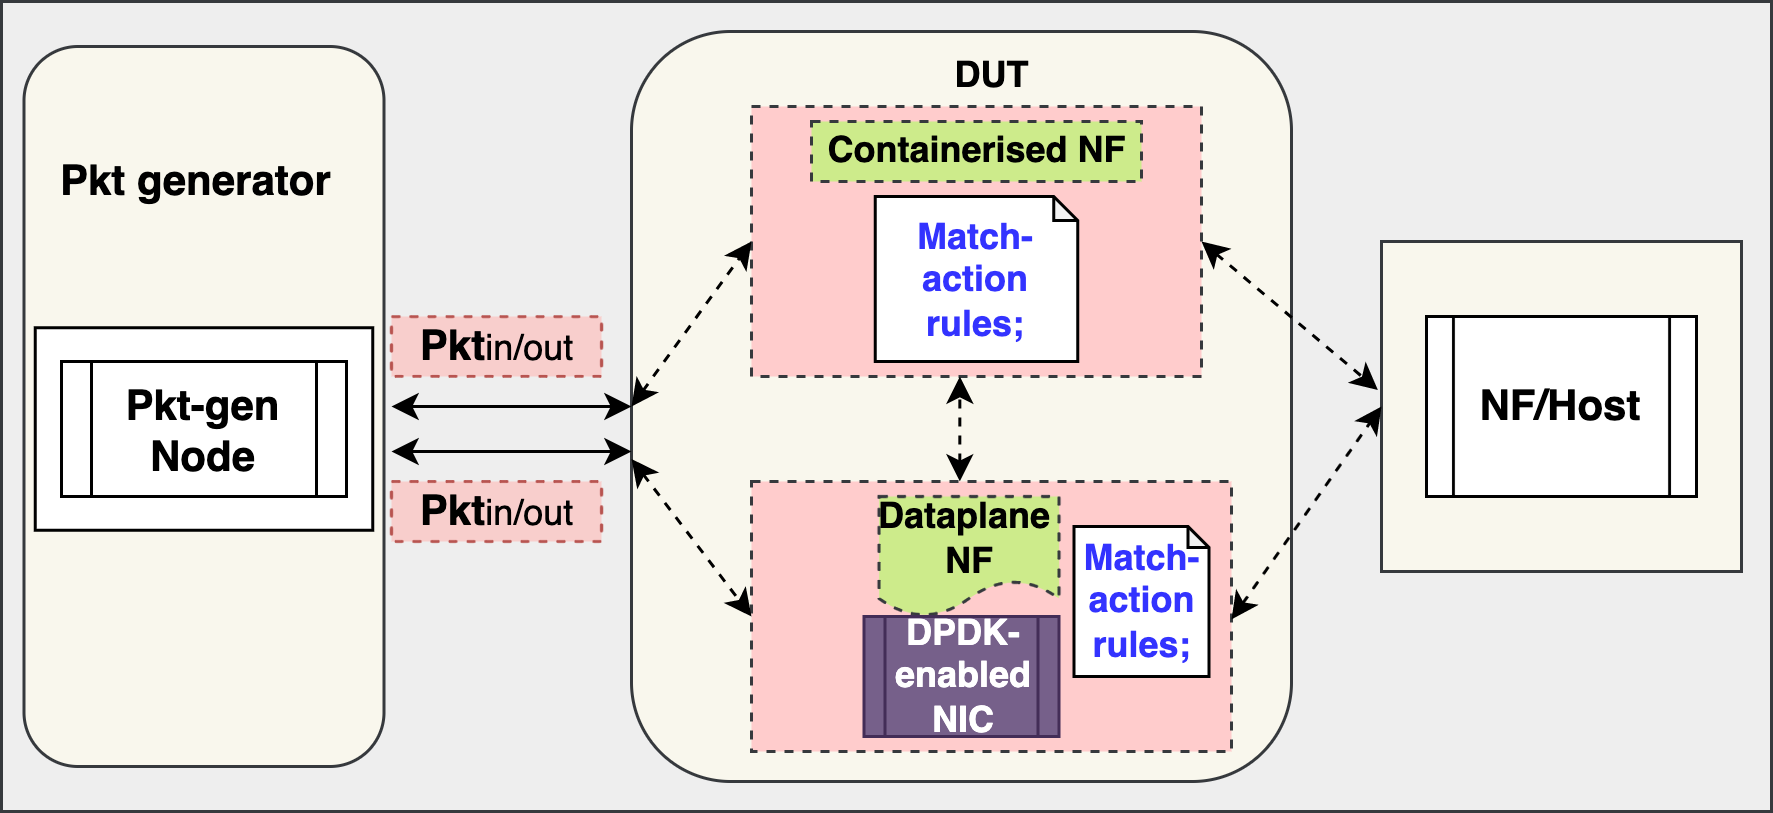
\includegraphics[width=0.92\columnwidth]{DPDK_Chain.png}
\caption{DPDK and Containerised NFs testbed - packets are generated and made to traverse the containerised NF or Dataplane NF at any given time. Match-action rules are inserted, based on type of functionality (a router or firewall function).}
\label{DPDK-Testbed}
\end{figure}
%%%%%%%%%%%%%%%%%%%%%%%%%%%%%%%%%%%%
This part of our evaluation leverages the OpenNetVM NFV framework, which is ideal for building high-speed vNFs that can handle line-rate packet processing using zero-copy and the DPDK poll-mode driver, rather than interrupts \cite{zhang2016opennetvm}. The OpenNetVM manager represents the NFV MANO component, as it is responsible for NF life-cycle management. We made use of a commodity servers (depicted in Figure \ref{DPDK-Testbed}), one as a packet generator with \texttt{pktgen} packet generator, the other as the Device Under Test (DUT), with network functions built on the OpenNetVM framework. The CPU on the DUT is an Intel(R) Core(TM) i7-8700 CPU @ 3.20GHz, with 6 cores (without hyper-threading), for improved performance per core. We made use of pktgen-dpdk\footnote[2]{https://git.dpdk.org/apps/pktgen-dpdk}, which generates packets at line-rate, and observe the packet processing rate per second, as packets are processed by the firewall NF. Note that our ability to scale the number of NFs in this part of our evaluation, depends on the number of available CPU cores, as each NF is assigned a single CPU core to run. As with the DPDK NFs, we also restricted our containerized NFs to run on single CPU cores for a fair comparison.



%%%%%%%%%%%%%%%%%%%%%%%%%%%%%%%%%%
\begin{figure}[ht]
\centering
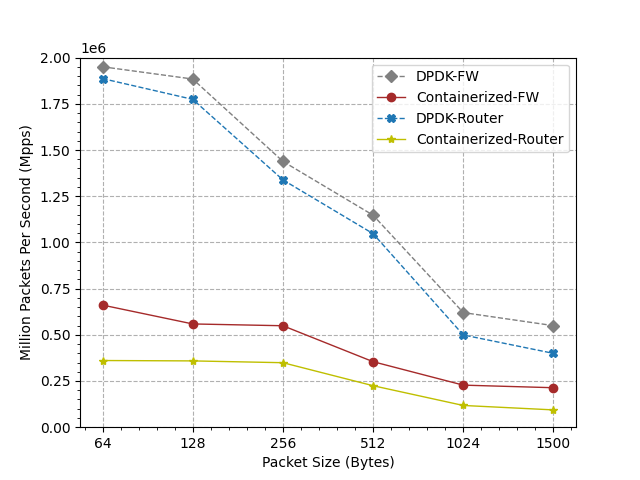
\includegraphics[width=0.9\columnwidth]{ContainerDPDK.png}
\caption{Million Packets Per Second -- DPDK and Containerized NF. The DPDK firewall NF processed about 2Mpps. All NFs are tied to separate CPU cores, for performance isolation and measurement consistency.}
\label{ContainerDPDK}
\end{figure}
%%%%%%%%%%%%%%%%%%%%%%%%%%%%%%%

We run the NFs as depicted in Figure \ref{DPDK-Testbed}, for the firewall NF scenario, we initialised the NF by creating an initial batch of 16,000 packets from the packet generator, which increases while the NF runs, and the packets are sent back to the RX queue of the generating NF (for measurements). This scenario was first carried out for the firewall NF, and using the router LPM NF. The results are as shown in Figure \ref{ContainerDPDK}, where the packets per second rates obtained are depicted for the minimum-sized (64B) and MTU-sized (1500B) packets.

%%%%%%%%%%%%%%%%%%%%%%%%%%%%%%%%%%%%%%%%%%%%%
%%%%%%%%%%%%%%%%%%%%%%%%%%%%%%%%%%%%%%%%%%%
\section{Discussion and recommendations}
\label{Discussion}
For us to fully appreciate how deployment choices by network operators can affect NFV performance, we carried out our evaluation with multiple physical commodity servers. Also, containerized and DPDK NF scenarios benefited from our design choice of running NFs on separate CPU cores.   

Another design consideration worth mentioning is the behaviour of NFs that are built using kernel-bypass frameworks such as the Intel DPDK library, the number of available CPU cores is especially relevant when service providers decide to adopt this approach. This is even more so as NFs are often tied to available cores, and depending on the scenario, some cores need to be made available for the NF manager or controller. 

In our first testbed (Figure \ref{OvS Testbed}), although this is not a claim that is generalizable for all dataplane implementations out there, the data-plane deployment consistently outperforms the user-space VNF when it comes to achieved bandwidth in the environment we have evaluated in our work. This is particularly noticeable with larger packet sizes, and more so in the case of the firewall VNF tests. This consistency also holds true for CPU utilization. By implication, service providers can leverage the data-plane of the network, especially in situations where compute-intensive NFs are deployed. The overall performance of network functions evaluated increased significantly using DPDK, even for 64B packets. Service providers can also leverage this for deploying compute-intensive vNFs such as a stateful IDS, for faster packet processing.

The mode of operation of some network functions in Table \ref{VNF-Table} such as WAN optimisers involves carrying out tasks such as traffic compression/decompression, caching, floating-point operations and sometimes content duplication \cite{he2022joint}. Such operations are not readily supported by current data-plane technology hence service providers can leverage other heterogeneous deployment options.


One of the practical scenarios that would benefit from the results of our work is a network service provider that provides a set of network functions comprising a gateway firewall and an Intrusion Detection System (IDS). This chain of network functions which are currently being implemented at the user-space of the network can be split in a hybrid manner between the data-plane and user-space to improve performance and reduce processing and service deployment costs. 

A network function such as an IDS which is stateful, requires the use of security modules, and is computationally intensive \cite{chen2022automatic}. This will benefit from the available resources (memory, CPU and I/O) at the user-space of commodity servers while having the firewall functionality or other lightweight functions deployed at the network data-plane. Also, in some existing and emerging Edge network use cases such as e-healthcare, self-driving cars and mixed reality (MR), depending on application profiles and requirements, a hybrid deployment scheme can be employed. We can achieve better performance by delegating simple, time-critical operations to the data-plane and leaving only more complex stateful and resource-hungry processing for user-space vNFs; which should also help eliminate processing redundancy.  


%%%%%%%%%%%%%%%%%%%%%%%%%%%%%%%%%%%%%%%%%%%%%%%%%%%%%%%%%%%%%%%%%%%%%%%%%%%%%%%%
\section{Related Work}
\label{Related Work}

The effect of having concurrent NFs run on a commodity server was characterized by Pitaev \textit{et al.} \cite{pitaev2018characterizing}, using OvS-DPDK, SR-IOV, and FD.IO VPP. They were able to show that having multiple VNFs deployed on a single host produces some performance bottlenecks, especially as the number of VNFs are increased. We evaluated our NFs implementation using two physical servers connected back-to-back, and report on some of the benefits of doing so. We carried out our experiments in the context of SDN, where match-action rules are inserted to the data-plane of virtual switches. 

Rasoul \textit{et al.} \cite{behravesh2019performance} evaluated the performance of virtualization technologies (unikernels, VMs and containers) for NFV deployments, with a focus on edge networks. They deployed two services (Redis and Apache) to examine the behaviour of these virtualization environments. They recommended the use of unikernels for applications with high context switching between userspace and kernel-space. VMs and containers demonstrated stable performance behaviour when compared to unikernels, with VMs having additional hypervisor overheads. We take a different approach by considering not only the effect of NF deployment on VMs and containers but using heterogeneous execution frameworks with commonly used network functions (a router and a firewall).

SDN-VNF performance was analysed by Gedia \textit{et al.} \cite{gedia2018performance}, in the context of VM and container implementations. They considered parameters such as CPU and memory utilization, service provisioning time and throughput. In their work, an ONOS SDN controller was deployed using containers and VMs, they attempted to answer a question that would help network operators in choosing the ideal platform for hosting VNF/SDN services. Their results show much better performance using the containerised NF approach. This informed our decision to further explore what is obtainable using a high performance packet processing approach such as DPDK and consider the implementation of NFs that incorporates the typical behaviour of middleboxes found in service provider environments rather than controllers. 


%%%%%%%%%%%%%%%%%%%%%%%%%%%%%%%%%%%%%%%%%%%%
%%%%%%%%%%%%%%%%%%%%%%%%%%%%%%%%%%%%%%%%%%%%
\section{Conclusions}
\label{conclusion}
We have evaluated the performance of different VNF implementation alternatives and motivate the deployment of network functions as part of the SDN-aware data-plane of the network for better service delivery, especially where latency-sensitive and bandwidth-intensive network functions are to be implemented. Two unique testbeds were carefully designed, to implement commonly used network functions (a firewall and a router) using the data-plane component of a production-grade virtual switch, and network functions deployed on separate virtualized processing elements. We also considered a high-performance scenario, by using DPDK and Docker containers for deploying the same network functions, which shows a significant increase in the performance of the network functions considered.

There are different ways in which this work could be built upon. Firstly, the dimensions of the evaluation can be extended by evaluating the data-plane scenario on a programmable hardware switch, which provides the option of offloading packet processing to SmartNICs, and also provides more in-network processing options, as these technologies are gradually gaining traction in service provider networks.
Secondly, we envisage hybrid deployment scenarios where service providers deploy NFs using both data-plane and user-space processing elements, depending on application profiles, NF complexity and resource availability in the network infrastructure. In such circumstances, the outcomes of our work can be used to build a knowledge base to be used by a deployment decision support system. 

%%%%%%%%%%%%%%%%%%%%%%%%%%%%%%%%%%%%%%%%%%%%%%%%%
\section*{Acknowledgments}
{This  work  was  supported  in  part  by  the  UK  Engineering and  Physical  Sciences  Research  Council  (EPSRC)  grant EP/N033957/1, the PETRAS National Centre of Excellence for IoT Systems Cybersecurity, which has been funded by the UK EPSRC under grant number EP/S035362/1, and the Petroleum Technology Development Fund (PTDF) Nigeria, grant 1563/19.}
%%%%%%%%%%%%%%%%%%%%%

\balance
\bibliography{bibREF.bib}
\bibliographystyle{IEEEtran}
\end{document}